\chapter{Models for the Delay}
\label{chapter4: Worm propagation}



The formalization of the FlipIt game with a delay relies on some value  \textit{d} that represents the time needed to infect a sufficient number of nodes in a network after the initial infection. This chapter provides the reader with more insight on how to calculate the value of this parameter \textit{d}.  \\

The spreading of malware has already been extensively researched. Because of the many different types of propagation methods it is hard to define a single model that can model all of them. Modelling the spread of malware depends on two key factors: the method used for the propagation and the graph of the network in which the malware will spread. \\
Viruses and worms are the two most researched types of malware.
 Since the spreading of viruses requires human interaction, their propagation delay depends on (hard to predict) human behaviour. Worms on the other hand, spread without human intervention, and their propagation is therefore easier to model. Since the purpose of this chapter is only to illustrate how a delay can be calculated, we will limit this chapter to propagation models of worms. \\

The overview of this chapter will be as follows: Section \ref{methodsofpropagation} presents an overview of the most frequently used propagation methods by worms. These propagation methods will be covered by different models in section \ref{modelsforpropagation}. A set of models is selected to illustrate the different possible ways to extract parameter \textit{d}. Section \ref{eigenmatrixmethode} introduces an easy method to calculate the propagation delay of a worm. In the last section \ref{googlesec:5.4}, a method based on the PageRank algorithm of Google is used to determine the probability of infection after a certain time period.%which node has a higher probability of being infected by a worm. % Different kind of graphs to model a computer network are introduced. 

%This chapter is based on the following papers: \cite{importantjournal}, \cite{OnWorms2005survey}, \cite{GameTheorApprCostBenefitAnalyses} and \cite{SecurelistAPT}.


\section{Methods of propagation}
\label{methodsofpropagation}

In the context of malware propagation, there are two kinds of APTs. First, there are APTs that launch an attack on just one target node of a network. The mechanism these APTs use to propagate malware is the dropper mechanism. The dropper is the initial attack vector that compromises the single targeted node of the system. The second kind of APTs target multiple nodes. These APTs also use a dropper mechanism but have an additional mechanism for self-propagation in order to propagate themselves to the multiple targeted nodes of the system. If the APT uses virus spreading, the virus infects one node on the network and has to wait for human interaction to spread. As such the spreading speed depends on the human interaction, and modelling virus propagation therefore requires modelling human behaviour. If an APT uses a worm propagation method it will spread by itself after it has been dropped on the network. Given the additional complexity of incorporating the human factor in a spreading method and that this chapter is merely meant as illustration on calculating the delay for use in the game theoretic approach, this chapter will be limited to worm propagation models for APTs. \\

Infection by worms start by dropping the worm on the network. Different dropping mechanisms can be used, whereby the initial attack can be random or targeted at a specific node. Frequently used mechanisms are USB sticks (given to a specific person or left behind to be picked up by a random person), email, or malicious software through phishing or trojan horses. To determine the total delay, however, the propagation strategy is of higher importance than the drop mechanism. The propagation strategy is used to determine the next nodes the worm will spread to. The following are common propagation methods: 
\begin{description}
%\item Scanning methods: A worm tries to guess (scan) the address of potential target nodes to infect. It can use distinct ways of scanning.
%% random, localized, topological or hit-list scanning.
%\begin{itemize}

\item \textbf{Selective Random scanning:} The worm randomly  selects a part of the selected IP address space instead of scanning the whole address space. The selected IP address space is a certain IP address area that the attackers are planning to attack. The reserved address blocks and the unassigned addresses are excluded from the address space. The rate of success for randomly chosen IP addresses is very low, but it is easy to implement. Example of such worms are \textit{Code Red} \citep{OwnInternetSI} and \textit{Slammer} \citep{moore2003inside}. 


\item \textbf{Localized scanning:} A worm that uses localized scanning will scan for hosts in the local address space. This method is used by the \textit{Code Red II} \citep{OwnInternetSI} and \textit{Nimda worm} \citep{OwnInternetSI}.
%\item \textbf{Topological scanning:} Address information stored in the victim machines are used to locate new targets. This method used by the `Morris' worm.

%\item \textbf{Hit-list scanning:} With the method of hit-list scanning, a short-list of vulnerable systems is made beforehand.  This is done to speed up the spread of worms at the initial stage. --This list consists of potentially vulnerable machines that are gathered beforehand and targeted first when the worm is released. An extreme case for the hit-list-scanning worms is a flash worm, which gathers all vulnerable machines into the list.--

\item \textbf{Sequential scanning:}
With sequential scanning, the worm will scan the IP addresses sequentially. This means that once a vulnerable host is compromised, it will look for IP addresses that are near to this host. For example, the address of the host is A, the next addresses that the worm will scan are A+1, or A-1. This method is used by the \textit{Blaster worm} \citep{zou2006performance}.
%-Remark -Stijn- Hier welke IP addressen worden er juist gescand? Alle of alleen lokale, niet echt duidelijk :) kan ook zijn dat het van de implementatie afhangt natuurlijk


\item \textbf{DNS random scanning:} Another strategy is a kind of strategy in which the DNS infrastructure is used to locate a new target address. The IP address table from a DNS server is acquired from DNS records. 
The speed of a DNS scanning worm in the IPv6 internet is comparable to the speed of an IPv4 random scanning worm. 
%There are some difficulties with this scanning technique. 
%First it is difficult to obtain the whole address space from the DNS records. Secondly, the worm has to carry the database, which can slow down the propagation if the database is to big. Last, t
The IP addresses stored in the address table are only hosts with public domain names. This propagation method is used by \textit{MyDoom} \citep{kamra2005effect}.

\item \textbf{Routable scanning:} The worms using routable scanning acquire target IP addresses based on the routing information in a network. Through  the BGP routing tables they can scan the routable address space. This method is three times faster than a traditional worm that uses random scanning. Examples are \textit{Spyb0t} or \textit{network Bluepill}. 
%--a ''routing worm'' [20]. Zou et al. designed two types of routing worms [20]. One type, based on Class-A (x.0.0.0/8) address allocations, is thus called 'ClassA routing worms.'' Such worms can reduce the scanning space to 45.3\% of the entire IPv4 address space. The other type, based on BGP routing tables, is thus called''BGP routing worms'' Such worms can reduce the scanning space to only about 28.6\% of the entire IPv4 address space.--
%\end{itemize}   

\item \textbf{Topology-based Worms:} Email and other client application worms: an email worms uses the email systems to find email addresses to propagate. Other client applications can include: Internet Relay Chat (IRC), Instant Messenger (IM), and a variety of peer-to-peer
file sharing systems, which have been used by worms to propagate in a similar way as email worms. For example, the \textit{Kak worm} \citep{Kakworm} is a JavaScript computer worm that spread itself by exploiting a bug in Outlook Express. % Another example is `GhostNet'

%Pikachu worm: The virus was mainly spread through Microsoft Outlook email attachments. The email containing the attached virus propagated through infected users by sending itself to all contacts in the user's Outlook address book. [5]
%\item \textbf{self stopping worm:} reduces speed to avoid detection. Atak worm or self stopping worm \cite{VirusChangePropSpeed}.
%\item \textbf{network sharing} `Shamoon'
%\item \textbf{shared files or spreading through SMB} (shared message block or  Common Internet File System (CIFS)) Flame
%\item \textbf{Zero-day vulnerabilities} \begin{description}
%\item Crouching Yeti is hardly a sophisticated campaign. For example, the attackers used no zero-day exploits, only exploits that are widely available on the Internet. But that did not prevent the campaign from staying under the radar for several years. \url{http://www.kaspersky.com/internet-security-center/threats/crouching-yeti-energetic-bear-malware-threat}
\end{description}

 Modelling the propagation methods described above can help us to find the time needed for a worm to infect the whole network. This will be equal to the \textit{d} parameter in the FlipIt model with propagation delay. \\

\section{Models for worm propagation}
\label{modelsforpropagation}
Early work on worm propagation models are based on the spread of real-world epidemic diseases. These models are based on the transition state of each node in the network.\\

%Scan based or Topology based
A node in a network can be in three different states: susceptible, infected or removed. A susceptible node is a node that is vulnerable to infection. An infected node is a node that has been compromised and can infect other nodes. A removed node is dead or immune, which means it cannot be infected again by worms. With these three states three main propagation models are proposed: SI (Suspected-Infected), SIR (Suspected-Infected-Removed) and SIS (Suspected-Infected-Suspected). In the SI model, a node that has once been infected, stays infected. In the SIR model, an infected node can be removed afterwards. This node cannot become infected again. In the SIS model a node can become susceptible again after it has been infected. Currently, various other models have been proposed based on these three models ( Wang et al. \cite{wang2014modeling}, Qing and Wen et al. \cite{OnWorms2005survey}, Xiang t al. \cite{xiang2009propagation} and Serazzi et al. \cite{serazzi2004computer}). We are only interested in models that will allow us to find the delay. \\ 


The most recent survey on common propagation methods is the one by Wang et al. \citep{wang2014modeling}. It encompasses the results of older surveys and explicitly focuses on propagation methods, while other papers also focus on other aspects such as  detection mechanisms and containment systems.
Table \ref{tree} provides the taxonomy on worm modelling, given in \citep{wang2014modeling} (only analytic modelling methods).
 All models that are based on the SI model type are appropriate, because in our model every node that is infected will stay infected. The other propagation models, SIR and SIS, are only interesting if there is a possibility to reduce the models to an SI model. The following section will extract the delay parameter from some of the models. These models are not meant as an exhaustive list, but rather as an illustration to the possible ways of extracting the delay out of an propagation model. 
%Only the Local Preference and Email worms models will not be explained because they involve human interaction. OSN model is done by means of simulation. The SIR AAWP model is also interesting because the parameter that involves the R part of the model can be deleted.  \\ \todo{laatste zinnen zijn wazig: Het deel erboven over SIS enzo was duidelijk maar hier worden andere modellen er bij de haren bijgesleurd. Als we die niet bekijken, gewoon kort zeggen dat er andere modellen zijn (e.g. SIR AAWP, Email worms, ....) maar dat deze niet worden bekeken ofzo?}



%The methods of propagation can be divided into different model types. SI, SIS and SIS... uitbreiden.. We are only interested in models that are based on SI model type (Susceptible-Infected), because in our model every node that is infected will stay infected. 


%The propagation models of diseases are applicable to the propagation of worms. SI, SIS and SIR. The SI model or also SEM (Simple Epidemic Model) is a model where the hosts in the network only have two states: Susceptible or Infected. Once they are infected they stay that way. The second model, SIS, is a model where the hosts can return to the Susceptible state, which in turn can become infected again. SIR is a model where the hosts can go in a Removed state. Once it is in a Removed state the hosts can not be infected any more. \\


%In this chapter we are only interested in the SI model. To apply the propagation models on FlipIt we need to know the propagation speed of the virus, without hosts becoming susceptible again. All hosts must stay infected. For this we only look at SI models. In table \ref{tree} the taxonomy of the propagation methods are given and the type of model. The General Epidemic model and Two-factor model are based on the Simple Epidemic Model with the difference that they both have extra parameters to model the Removed state.  We discuss a couple of SI models and then introduce a method of out own.\\



%In this section we only list the models that are the most interesting from the perspective of calculating the delay, namely the SI type models.
%SI, SIR, SIS assume $\beta$ to be constant.

%Tree model figure \ref{tree}. We introduce homogeneous models. Network topology is mixed. 

\begin{figure}
\centering
%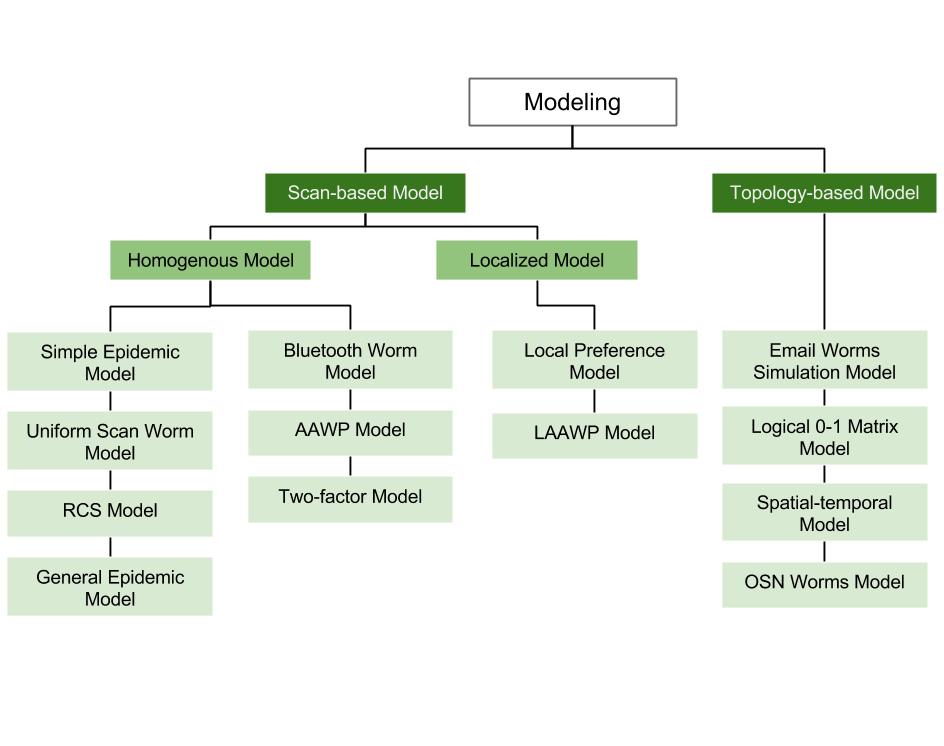
\includegraphics[scale=0.4]{Images/tabel3.png} 
%\caption{Taxonomy of worm modelling. Image based on taxonomy given in \cite{wang2014modeling}}.
%\label{tree}
%\end{figure}
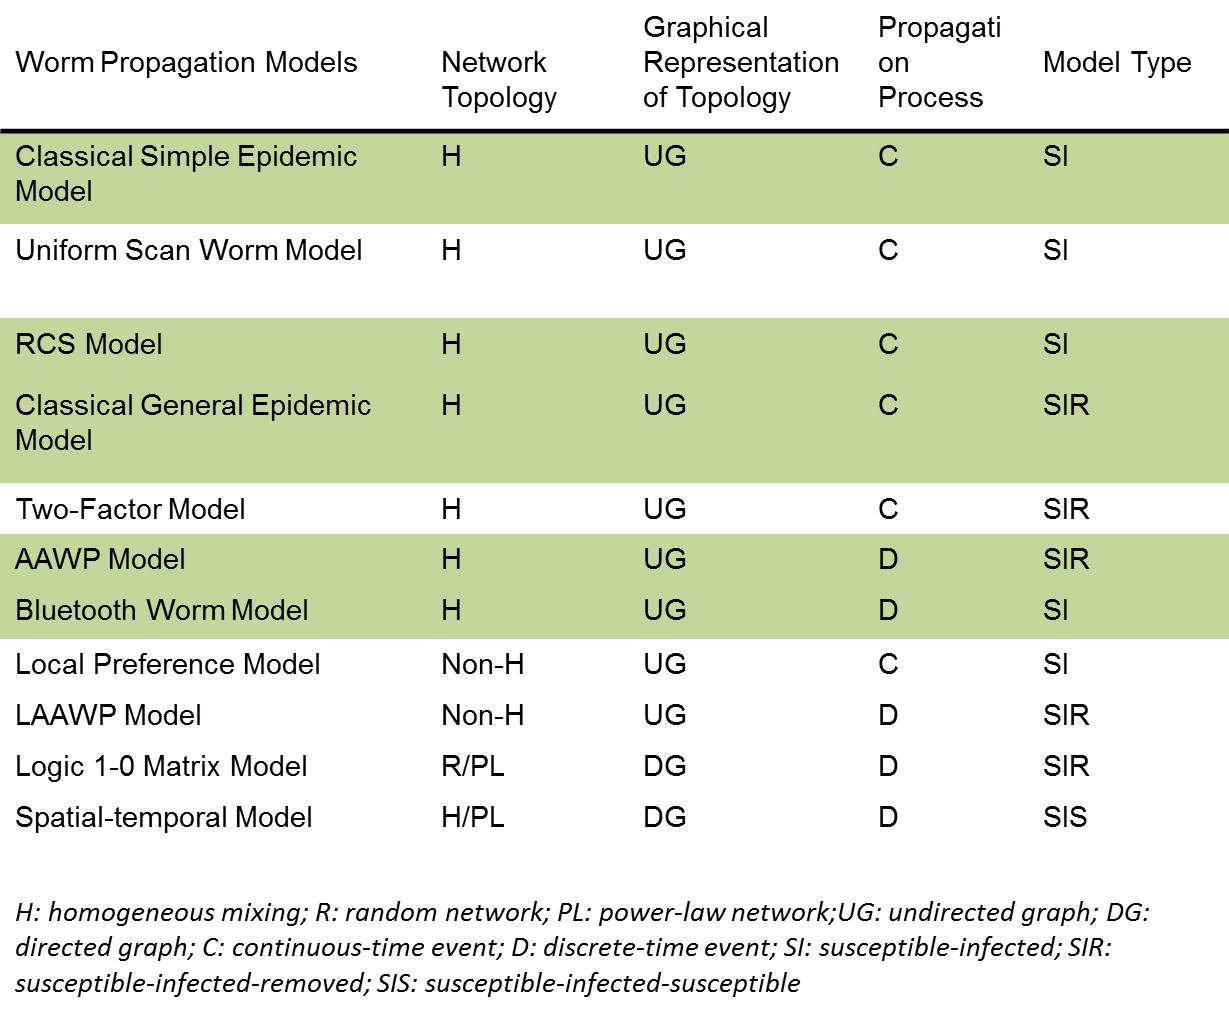
\includegraphics[scale=0.55]{Images/Picture2.png}
\caption{Taxonomy of worm modelling.Table based on only analytic worm propagation models given in \cite{wang2014modeling}. The models in green are the models illustrated in this paper.}
\label{tree}
\end{figure}



\subsection{Simple Epidemic Model}
%Codered paper gebruikt voor model
A Simple epidemic model is another name for the general SI model. This model assumes that each node in the network can be either susceptible or infected. 
Once a node is infected it will stay infected. Every node in the network has the same chance to be infected. 
The simple epidemic model is considered to be of a fixed size, meaning that no nodes are added to the network or removed. The model for a fixed population is as follows:

\begin{equation}
\dfrac{d I(t)}{dt} = \beta I(t)[N-I(t)]
\end{equation} 
where \textit{I(t)} is the number of infected nodes at time \textit{t}, $\beta$ is the propagation rate, and \textit{N} is the number of nodes in the network. In the beginning, $t=0$, \textit{I(0)} nodes are infected. All the other nodes, $N - I(0)$, in the network are susceptible. 
The solution of this equation is the following logistic curve:
\begin{equation}
I = \dfrac{e^{\beta(t-T)}}{1+e^{\beta(t-T)}}
\label{SIdelay}
\end{equation}
where \textit{T} is a time parameter representing the point of maximum increase in the growth.\\

%-Remark- Stijn- prentje van de curve maar hoeft niet
%\begin{figure}[hbtp]
%\centering
%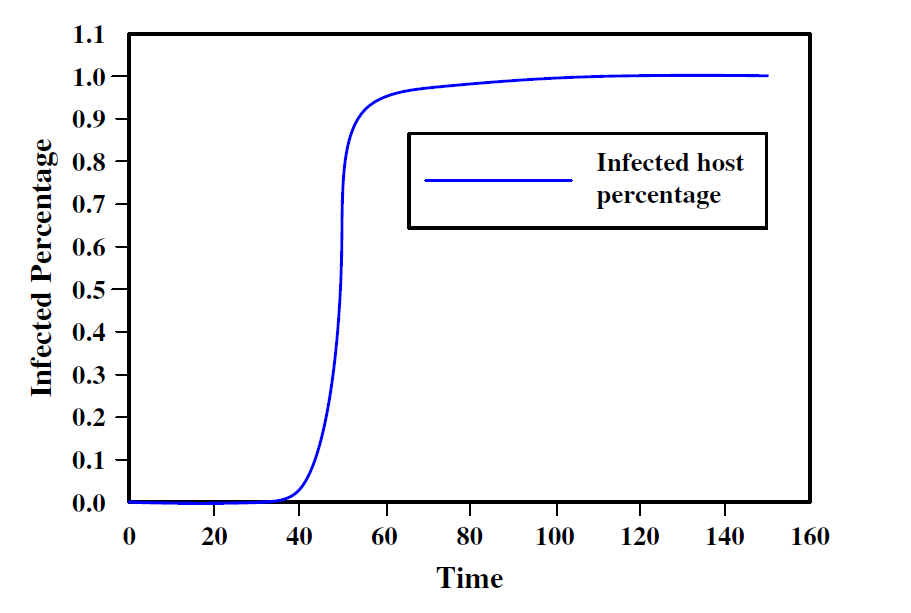
\includegraphics[scale=0.5]{Images/SEMmodel.png}
%\caption{Simple Epidemic Model. The x-coordinate is the propagation time and the y-coordinate is the infected percentage of the whole network. Original image from \cite{OnWorms2005survey}}
%\label{SEMmodel}
%\end{figure}

%Figure \ref{SEMmodel} laat het SEM model zien.
%This simple epidemic model has been used in various papers \cite{OwnInternetSI}, \cite{CodeRed} to model random scanning worm such as \textit{Code Red} and \textit{Slammer}. \\
%For our paper we have to approximate the propagation speed en Infect gelijkstellen aan het aantal genoeg nodes die geinfecteerd moeten zijn door de APT om de controle te hebben. Dan weten we hoelang het duurt. In het begin zullen er ook geen geinfecteerde hosts zijn, dus de vergelijking kan opgelost worden.\\
%%Er wordt geen rekening gehouden met de topology ? nog uitzoeken.
To extract the delay from the formula we need the total number of nodes in the network. If \textit{I} in formula \ref{SIdelay} equals the total number of nodes, variable \textit{t} will be the value of the delay that we need. A limitation of this model is that it is only applicable to nodes in a homogeneous network. A homogeneous network is a network where every node has approximately the same degree, the number of connections the node has. This model is thus suitable for propagation of worms that are topology independent (e.g scan-based worms), because every node has the same chance to be infected by another node in the network. The \textit{Code Red} worm, which is a random scan based worm, has been analysed by this kind of model in \cite{OwnInternetSI}. Another limitation is that the graph is presented as an undirected graph. This means that the spread can always happen in both ways, which may not be suitable for every worm propagation. 

%-Remark -Stijn- begreep degree niet van nodes en topology independent
\subsection{RCS model}

The RCS model stands for Random Constant Spread model and was developed by Paxson and Weaver at Stanford \citep{OwnInternetSI}. It is a model derived from the classical Simple Epidemic Model and was used to analyse the \textit{Code Red I} worm. For this model it is assumed that the worm owns a good random number generator that is properly seeded. \\

Let\textit{ N} be the total of vulnerable hosts in the network that can be potentially infected. It is assumed that no system is patched, shut down, deployed or disconnected. This means that the number of hosts in the system stays constant. 
%The model also ignores a sudden spreads of the worm behind firewalls on private networks, because this can be misleading. \todo{wat betekent de laatste zin?}
Let K be the initial compromise rate. This is the rate per hour at which the worm can find and compromise hosts at the beginning of the infection. \textit{K} is a global constant and therefore does not depend on the speed of the network or the processor speed.  Every machine can infect only one other machine after it has been compromised. The rate that a worm can find hosts can not be increased. 
Let \textit{T} be the moment of the start of the infection. Variable \textit{a} is the proportion of vulnerable hosts that has been compromised. Variable \textit{t} is the time in hours. \\

The formula to model the spread of the worm is as follows:
\begin{equation}
N da = (N a)K(1 - a)dt
\end{equation}
It tells how many vulnerable machines will be compromised in the next amount of time \textit{dt}, when the proportion of the machines \textit{a} that are already compromised is known.\\

From this, it follows the simple differential equation:
\begin{equation}
\dfrac{d a}{dt} = Ka(1-a)
\end{equation}
With the following solution:
\begin{equation}
a = \dfrac{e^{K(t-T)}}{1+e^{K(t-T)}}
\end{equation}
\\

To extract the delay from this formula, we need to know the maximum numbers of hosts that can be infected before the total system is compromised. The initial compromise rate has to be approximated. \textit{t} is the time variable. If \textit{a} passes the proportion of nodes that have to be compromised before the whole system is compromised by the attacker, value \textit{t}  is the value of \textit{d} in the FlipIt game with propagation delay.\\

A drawback of this model is that the network topology is assumed to be homogeneous and that the paths between the nodes are undirected. 
%-Remark- toevoeging van mama:
%An example would be the Internet, since the topology of the Internet is considered to be a complete undirected graph. The RCS model is an SI model and therefor the state of a host can only be syspected or infected. Once a node has been compromised it stays that way. Finally, the model also ignores the spreading of worms behind firewalls on private networks.

%\subsubsection{Kermack-Mckendrick model: SIR}
%In the Kermack-Mckendrick model, also known as SIR model, nodes can have three states: susceptible, infected or removed. Once a node of the network has been recovered from a worm, the node will stay in the removed mode and never becomes infected again. These nodes are not able to infect other nodes and can no longer be infected. \\
%Let I(t) be the number of infectious hosts at time \textit{t}, R(t) be the number of removed hosts at time \textit{t} and J(t) is the number of infected hosts by time \textit{i}, regardless the fact that a node can be in a removed state.
%\begin{equation}
%J(t) = I(t) + R(t).
%\end{equation} 
%The Kermack-McKendrick model can be represented as follows:
%\begin{equation}
%\begin{Bmatrix} \dfrac{d J(t)}{dt} = \beta J(t) \big[N- J(t) \\
%\dfrac{d R(t)}{dt} = \gamma I(t) \\
%J(t) = I(t) + R(t) = N - S(t)
% \end{Bmatrix}
%\end{equation}
%Parameter $\beta$ is again the rate of infection and $\gamma$ is the rate of removal of infected hosts. S(T) is the number of susceptible hosts at time t.
%\begin{figure}[hbtp]
%\centering
%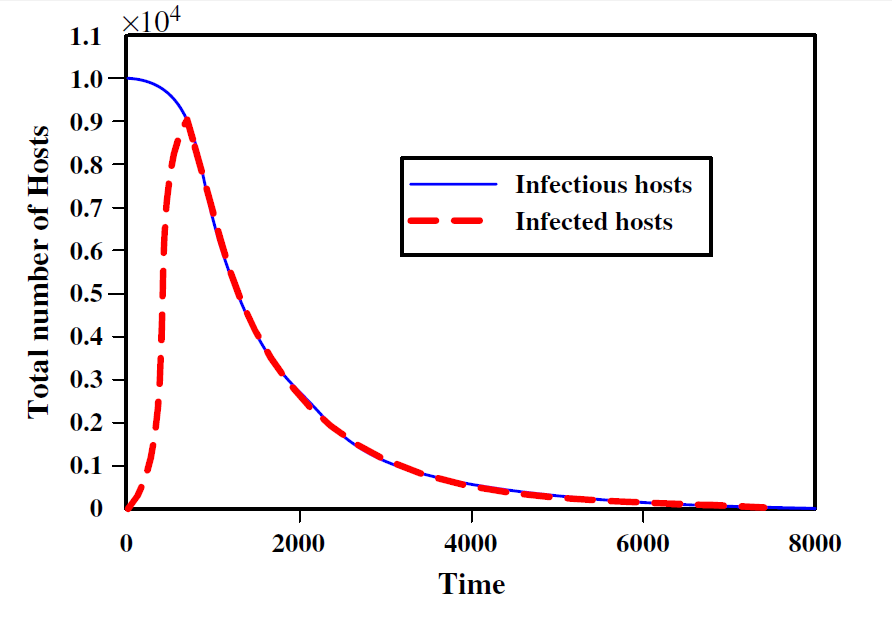
\includegraphics[scale=0.5]{Images/KMmodel.png}
%\caption{KM Model. The x-coordinate is the propagation time and the y-coordinate is the infected percentage of the whole network. Original image from \cite{OnWorms2005survey}. $N=10000, \beta = 1/10000000$.}
%\label{KMmodel}
%\end{figure}
%
%%codered%
%--Define $\rho = \gamma/\beta$ to be the relative removal rate [3]. One
%interesting result coming out of this model is
%dI(t)
%dt > 0 if and only if S(t) > p. (6)
%Since there is no new susceptible host to be generated,
%the number of susceptible hosts S(t) is a monotonically decreasing
%function of time t. If S(t0) < p, then S(t) < p and
%dI(t)/dt < 0 for all future time t>t0. In other words, if the
%initial number of susceptible hosts is smaller than some critical
%value, S(0) < p, there will be no epidemic and outbreak
%[15].
%The Kermack-Mckendrick model improves the classical
%simple epidemic model by considering that some infectious
%hosts either recover or die after some time. However, this
%model is still not suitable for modeling Internet worm propagation.
%First, in the Internet, cleaning, patching, and filtering
%countermeasures against worms will remove both susceptible
%hosts and infectious hosts from circulation, but KermackMckendrick
%model only accounts for the removal of infectious
%hosts. Second, this model assumes the infection rate
%to be constant, which isn't true for a rampantly spreading
%Internet worm such as the Code Red worm--
%
%%\subsubsection{Two-Factor model}
%%%distributed worm simulation
%%--Zou et
%%al. [15] present a ''two-factor'' model that extends SIR
%%epidemiological model to capture the effects of human
%%countermeasures and the congestion due to the worm
%%spread. Shen et al. [16] provide a discrete-time worm
%%model that considers patching and cleaning effect and can
%%model worms with local scanning techniques. All these
%%approaches abstract specifics of the Internet topology,
%%change in the size of vulnerable population as the worm
%%spreads, and the effect of the individual host and network
%%defenses (except for patching, in case of [16]) on the
%%spread--
%\subsection*{self disciplinary worms}
%Model for self disciplinary worms and counter measures ... []  \$•${verder uitwerken ? ja of nee? }


%Popular mechanism that worms use to detect vulnerable targets by random IP scanning probing. Feasible due to use 32-bit addresses. 128-bit addresses life harder for worms, except the ones that use email systems to propagate. two new strategies: uniformly distributed random number generator to select new target. :spread locally, by biasing the search space towards addresses within the same subnet or network.  
%The second strategy is almost the same as what email virusses would get. For this reason we work an example out .. 
\subsection{Bluetooth worm model}

The Bluetooth worm model was introduced by Yan and Eidenbenz \citep{yan2009modeling}. The model captures the behaviour of the propagation of a worm that spreads through the Bluetooth protocol. 
A Bluetooth device that is compromised can only infect neighbour devices that are in its radio range.
Let \textit{i(t)} be the average density of infected hosts in the network at time $t_{0}$. Then: 
\begin{equation}
i(t_{k+1})=i(t_{k}) \cdot \dfrac{\rho(t_{k})}{i'(t_{k}) + (\rho(t_{k}) - i'(t_{k}))e^{-\alpha' \cdot \rho(t_{k}) / (\rho(t_{k}) - i'(t_{k}))}}
\end{equation}
where $\rho$(t) and $\beta$(t) are the average device density and the pairwise infection rate at time \textit{t} respectively. The number of new infections out of the infection cycle is denoted by $\alpha$(t). $\alpha'$ is used for a better estimation of the worm propagation, because the growth rate of the worm can change and this can maybe result in an overestimation of the number of new onfections. $\alpha'$ is determined as follows:
\begin{equation}
\alpha'=\dfrac{\rho(t_{k})-t(t_{k})}{\rho(t_{k})} \cdot \alpha(t_{k}) + \dfrac{i(t_{k})}{\rho(t_{k})} \cdot \alpha(t_{x})
\end{equation}

To apply this model on FlipIt we again set up a threshold value for i(t) and see how long it takes to compromise this amount of hosts.  The paper by Yan and Eidenbenz concluded in their work that after setting model parameters accordingly ($\lambda_{ne} = 0.2108$ the average node degree and $J_{in}= 0.2372$ the average meeting rate of neighbours), the model predicts that the time it would take to infect 99$\%$ of the devices is slightly less than one hour. So in this case the delay is equal to an hour and the amount of hosts that has to be infected by the attacker before the network is compromised is 99$\%$ of the hosts in the network.
The Bluetooth worm spreads rapidly once the density of the infected hosts reach 10 percent. The model shows that the spread in the beginning is very slowly at en early stage.\\

%-Remark -Stijn- waarom 99 procent en niet 100? gewoon een uitleg in de trant van bij 99 procent kunt ge even goed zeggen dat heel het netwerk geinfecteerd is is goed. Of mss is er effectief een reden in de paper genoemd voor de 99 
The limitation of this model is that it assumes that all the hosts in the network are homogeneously mixed and that the time increases in a discrete fashion. The graphical representation is also a undirected graph.

%\subsubsection{OSN worm model}
%OSN worms stands for Online Social Network worms. This model is based on worms that propagate through the use of social media, like Facebook. The difference between an email worm and a social network worms is that the topology of the network is different. 

\subsection{AAWP model}
AAWP stands for Analytic Active Worm Propagation. The model was proposed in \cite{chen2003modeling} by Chen et al. to model the discrete behaviour of a worm. The AAWP model is a SIR model which uses a death and patch rate to calculate the amount of hosts that become Removed. Yet this model can still be useful to calculate the delay because if the death and patch rate are removed, this model becomes an SI model. It is different from other SI models because it includes the time that it takes to infect a host. A host cannot infect another hosts before it is completely compromised. The model also considers the fact that a host can be scanned and hit by multiple worms at the same time. \\%This model is used for worms that propagate through uniform scanning. When uniform scanning is used, each IP address 

The spread of the AAWP model with death and patch rate is characterized as follows:
\begin{equation}
I_{t+1}=(1-d-p)I_{t}+[(1-p)^{t})N-I_{t}][1-(1-\dfrac{1}{\Omega})^{sI_{t}}]
\end{equation}
where \textit{d} is the death rate, $p$ is the patch rate, $I_{t}$ is the amount of infected hosts at time \textit{t}, \textit{N} is the number of vulnerable hosts, \textit{s} is
the scanning rate of the worm and $\Omega$ is the scanning
space. 

The spread of the worm without the death and the patch rate is as follows:
\begin{equation}
I_{t+1}=I_{t}+(N-I_{t})[1-(1-\dfrac{1}{\Omega})^{sI_{t}}]
\end{equation}

The iteration procedure with death and patch rate will stop when all the nodes in the network are infected or when the number of infected nodes remains the same. When the death and patch rate are removed from the formula the iteration procedure will stop when all the nodes are infected. So when the iteration procedure stops the delay will be equal to \textit{t+1}. \\


The biggest limitation of the model is that is expressed in discrete time. Continuous models are more appropriate for large scale models. The model also uses a complete undirected graph.


%Popular mechanism that worms use to detect vulnerable targets by random IP scanning probing. Feasible due to use 32-bit addresses. 128-bit addresses life harder for worms, except the ones that use email systems to propagate. two new strategies: uniformly distributed random number generator to select new target. :spread locally, by biasing the search space towards addresses within the same subnet or network.  
%The second strategy is almost the same as what email virusses would get. For this reason we work an example out .. \\



%A method to calculate the propagation of the virus in an easy way. Google page ranking algorithm. 


\section{Matrix worm model}
\label{eigenmatrixmethode}

As can be seen in table \ref{tree} all propagation models depend on a specific network topology. A distinction is made between four kinds of network topologies: homogeneous, non-homogeneous, random network or power-law network. A homogeneous network is a network where every node has about the same degree of connectivity and each connection has the same probability. A non-homogeneous network is a network in which not all the nodes have the same degree and the connections have a different probability.
%A small-world topology is a network where most nodes are not connected with each other but they can all reach each other in a few steps. Social networks are an example of such a small-world network. 
A random network is a topology in which each connection is chosen at random with equal probability. In a power law network the degrees of each node in the network follow the power law. Some of the nodes have a small degree of connectivity, others have a very large degree of connectivity.\\

However, for some of the propagation methods, the actual graph of the network matters. Each propagation method depends on having the right topology. Email worms need a topology that correspond to a social network, BGP routing worms need a topology on IP-network level. 
Ideally, the propagation delay should be calculated without assuming that the network has one of these predefined topologies, but rather using the actual topology of the network at hand. \\

%All of the above models for modelling the mechanism of the spreading of a worm depend on the kind of topology of the network.  
This chapter proposes a method to calculate the spread of a worm in a way that allows easy integration of the network topology. This method approximate how fast a worm can infect a network. It is capable of calculating the delay for any network topology. 


\subsubsection{Proposal of a matrix based model}
%-Remark -Stijn- Ik vind de matrices maar weinig zeggen ik snap dat ze nodig zijn maar misschien kunt ge de overeenkomstige graph erbij tekenen of een pad erin uitlichten in kleur. bvb wie node 1 allemaal geinfecteerd heeft. Maar misschien is dat ook niet nuttig. Ik zou mij hier niet te veel van aantrekken


%--iets zeggen dat het ook belangrijk is voor de defender om zijn netwerk zo aan te passen dat het virus moeilijker kan verspreiden. Network segregation mss aanhalen ?--
%
%\begin{description}
%\item Power law
%\item Small world topology
%\item random graph
%\item ..
%\end{description}

%The usefulness of this method is that it is graph model independent. The topology of the network has to be in the form of a square matrix. Each connection is determined by the entries on the matrix. 
%$N_{0}$ denotes the initially infected resources at the beginning of the virus propagation. 
%$P_{x}(R_{n},t|R_{0},r,t_{0})$ denotes the chance that resource $R_{n}$ is infected at time $t$ after dropping virus number x on to resource $R_{0}$ at $t_{0}$ with rate $r$. \\

%$S(R_{n},R_{0})$ denotes the shortest path from the infected resource $R_{0}$ to resource $R_{n}$. It gives back a value with the distance measured with how many resources are in between including the end resource. \\

%So the chance that a resource is infected after time t is the chance that the resource is infected by all the previous infections and that the defender has not flipped the resource.

A computer network can be modelled by an undirected or directed graph $G = < N, E> $ where $|N|$ denotes the number of nodes in the network and $|E|$ the number of connections. This graph can be converted to an  $|N| \times |N|$ adjacency matrix in which the entries represent the connections between the nodes of the network. \\
The matrix has a non-zero entry $a_{ij}$ if there is a connection from node $N_{i}$ to $N_{j}$. \\ 


Adjacency matrices have many interesting applications, amongst which calculating the paths between vertices:
\textit{``If \textit{A} is the adjacency matrix of the directed or undirected graph \textit{G}, then the matrix $A^{n}$ (i.e., the matrix product of \textit{n} copies of \textit{A}) has an interesting interpretation: the entry in row \textit{i} and column \textit{j} gives the number of (directed or undirected) walks of length \textit{n} from vertex \textit{i} to vertex \textit{j}. If \textit{n} is the smallest nonnegative integer, such that for all i ,j , the (i,j)-entry of $A^{n} > 0$, then n is the distance between vertex i and vertex \textit{j}.''}  source: \cite{wikimatrix} .\\
Using this property of an adjacency matrix, it is possible to calculate the time it takes for a worm, starting on a specific node, to infect a sufficient amount of other nodes in the network. Every matrix $A^{n}$ has a non-zero \textit{ij}-entry , if the worm starting in node \textit{i} can reach node $j$ in \textit{n} time steps. If we sum up all the matrices $A^{1} + A^{2} + ~...~+ A^{n-1}+A^{n}$, every \textit{i}-row indicates which node \textit{j} is infected by node \textit{i} after time $t=n$.  

%%% Local Variables: 
%%% mode: latex
%%% TeX-master: "thesis"
%%% End: 
\begin{figure}
\centering
\begin{tikzpicture}[->,>=stealth',shorten >=1pt,auto,node distance=2.8cm,
                    semithick]
  \tikzstyle{every state}=[fill=black!60!green,draw=none,text=white]

  \node[state] (A)                    {$N_1$};
  \node[state]         (B) [above right of=A] {$N_2$};
  \node[state]         (D) [below right of=A] {$N_3$};
  \node[state]         (C) [below right of=B] {$N_4$};
  \node[state]         (E) [below right of=C] {$N_5$};
  \node[state]		   (F) [above right of=C] {$N_6$};

  \path (A) edge              node {} (B)
            edge              node {} (D)
        (B) edge              node {} (A)
        (C) edge              node {} (B)
            edge 			  node {} (F)
        (D) edge 			  node {} (C)
        (F) edge 			  node {} (E);
\end{tikzpicture}
\caption{Network with 6 nodes. The arrows represent the connections between the nodes. }
\label{netwerkfiguur}
\end{figure}

%\[
%\begin{bmatrix}
%    x_{11}       & x_{12} & x_{13} & \dots & x_{1n} \\
%    x_{21}       & x_{22} & x_{23} & \dots & x_{2n} \\
%    \hdotsfor{5} \\
%    x_{d1}       & x_{d2} & x_{d3} & \dots & x_{dn}
%\end{bmatrix}
%=
%\begin{bmatrix}
%    x_{11} & x_{12} & x_{13} & \dots  & x_{1n} \\
%    x_{21} & x_{22} & x_{23} & \dots  & x_{2n} \\
%    \vdots & \vdots & \vdots & \ddots & \vdots \\
%    x_{d1} & x_{d2} & x_{d3} & \dots  & x_{dn}
%\end{bmatrix}
%\] 
Assuming a network like in figure \ref{netwerkfiguur}, the corresponding adjacency matrix is the  matrix $A$: \\

\begin{equation}
A =
\bordermatrix{
         & N_1		& N_2	& N_3	& N_4 	& N_5	&N_6     \cr
    N_1   & 0		& 1		& 1		& 0		& 0		& 0	     \cr
    N_2   & 1		& 0		& 0		& 0		& 0		& 0	     \cr
    N_3   & 0		& 0		& 0		& 1		& 0		& 0	     \cr
    N_4   & 0		& 1		& 0		& 0		& 0		& 1	     \cr
	N_5   & 0		& 0		& 0		& 0		& 0		& 0	     \cr
	N_6   & 0		& 0		& 0		& 0		& 1		& 0	     \cr
}
\end{equation}

In matrix $A \times A = A^{2}$, each entry represents the number of  paths with length 2 from $N_{i}$ to $N_{j}$:\\


\begin{equation}
 A \times A = A^{2} =
\bordermatrix{
         & N_1		& N_2	& N_3	& N_4 	& N_5	&N_6     \cr
    N_1   & 1		& 0		& 0		& 1		& 0		& 0	     \cr
    N_2   & 0		& 1		& 1		& 0		& 0		& 0	     \cr
    N_3   & 0		& 1		& 0		& 0		& 0		& 1 	     \cr
    N_4   & 1	    & 0		& 0		& 0		& 1		& 0	     \cr
	N_5   & 0		& 0		& 0		& 0		& 0		& 0	     \cr
	N_6   & 0		& 0		& 0		& 0		& 0		& 0	     \cr
}
\end{equation}

Likewise, in matrix $A^{2} \times A = A^{3}$ each entry represents the number of paths with 3 steps from $N_{i}$ to $N_{j}$.\\


\begin{equation}\label{5:13}
 A \times A \times A = A^{3} =
\bordermatrix{
         & N_1		& N_2	& N_3	& N_4 	& N_5	&N_6     \cr
    N_1   & 0		& 2		& 1		& 0		& 0		& 0	     \cr
    N_2   & 1		& 0		& 0		& 1		& 0		& 0	     \cr
    N_3   & 1		& 0		& 0		& 0		& 1		& 0	     \cr
    N_4   & 0		& 1		& 1		& 0		& 0		& 0	     \cr
	N_5   & 0		& 0		& 0		& 0		& 0		& 0	     \cr
	N_6   & 0		& 0		& 0		& 0		& 0		& 0	     \cr
}
\end{equation}


~~\\
So, in $A^{n}$ every $a_{ij}$ entry gives the number of paths with \textit{n} steps from $N_{i}$ to $N_{j}$.\\

Calculating the sum of the three matrices $(A + A^{2} + A^{3}) $ results in a matrix where the non-zero entries $a_{ij}$ indicate which nodes are infected after 3 time steps if a virus is dropped on noded \textit{i}:

\begin{equation}
 A + A^{2} + A^{3} = \sum A^{n} =
\bordermatrix{
         & N_1		& N_2	& N_3	& N_4 	& N_5	&N_6     \cr
    N_1   & 1		& 3		& 2		& 1		& 0		& 1	     \cr
    N_2   & 2		& 1		& 1		& 1		& 0		& 0	     \cr
    N_3   & 1		& 1		& 0		& 1		& 1		& 1	     \cr
    N_4   & 1		& 2		& 1		& 0		& 1		& 1	     \cr
	N_5   & 0		& 0		& 0		& 0		& 0		& 0	     \cr
	N_6   & 0		& 0		& 0		& 0		& 1		& 0	     \cr
}
\end{equation}

For this sample network, the matrix in \ref{5:13} indicates that by dropping a virus on node $N_{1}$, all but node $N_{5}$ will be infected after 3 time steps. If the virus is dropped on node $N_{5}$, the virus will not spread. \\

With the formula $\sum A^{n}$ the average delay can be calculated by counting the expected delay of every node when a worm has been dropped and devide it by the number of nodes in the network. \\

Matrix \textit{A} can also represent a graph where every link has a weight. The weight is equal to the probability that the worm spreads through that link. The outcome of $ \sum A^{n}$ is then equal to the probability that each node has been infected after n time steps. The average delay can be calculated by setting a threshold value for the probability that a node is infected. \\

\subsubsection*{Conclusion}
The advantage of this matrix worm model in comparison with the above models is that matrix  \textit{A} can represent any network topology, directed or undirected. \\
Using this method it is also possible to determine the shortest path through al the nodes in the network. The shortest path that is necessary to infect all nodes can be found by summing all the matrices. The first row that only has non-zero entries determines this path. From node \textit{i} to the last \textit{ij}-entry that became a non-zero value. Consequently, if a worm is dropped on node \textit{i}, this worm will compromise the network in the shortest time possible. A defender can use this knowledge to adapt its network configurations. \\
These matrix calculations may seem very time consuming, but in the domain of network analytics efficient algorithms are available that are capable of calculating network attributes per node in networks of millions of nodes. This paper only provides a proof of concept of how to apply these matrices to calculate the delay. Developing an efficient algorithm is considered as a potential avenue for further research. 
%Using this knowledge we can calculate in how many steps a node is infected: \\
%The infection vector or start vector $I_{0}$ of length $|V|$ indicates which node is infected and which not. Multiplying the infection vector with $A$ results in a vector $I_{1}$, which represents which nodes are infected after 1 step. Multiplying the start vector $I_{0}$ with $A^{N}$ calculates which nodes are infected in \textit{N} steps: each non zero entry represents an node infected after \textit{N} steps. \\
%In the context of the FlipIt game, it is safe to assume that once a node is infected, it stays infected until the defender Flips the node. This means that after d steps, it is assumed that all nodes that could be reached in less than \textit{d} steps from the node where the worm was dropped, are infected. In order to know how many nodes are infected after (for example) at most 3 steps, we have to consider nodes that are infected initially (step 1), or after 2 steps, or after 3 steps.  Calculating the sum of the three matrices $(A + A^{2} + A^{3}) $ results in a matrix that indicates for each node, the number of paths of length 1, 2 or 3 from \textit{i} to \textit{ j}. Multiplying the start vector with this matrix, results in a vector that indicates which nodes will be infected in at most 3 steps . This technique can be applied to calculate the state of the network after any number of steps. \\
%
%Determining the length of the delay boils down to determining which configuration of infected nodes is considered as corresponding to the attacker having flipped the resource. It may be that all nodes need to be flipped, a sufficient amount of nodes, or a (set of) particular nodes.\\
%
%--Hier nog een beetje verder uitschrijven hoe je exact de d dan moet bepalen, gegeven dat je niet weet in welke knoop het virus gedropt wordt-- \\


%What do we need for an algorithm
%\begin{description}
%\item Graph network $G = < V, E>$
%\item Graph matrix $[A]$ which is $|V| \times |V| $
%\item Attack vector $[X]$ which is $1 \times |V|$
%\item cummulative matrix $[M]$ which is $|V| \times |V|$
%\item state matrix $[T]$  which is $|V| \times |V|$
%\item Reset vector $[R]$
%\item duration \textit{d}
%\item time \textit{n}
%\item rate $\delta _{0}$ of defender and $\delta _{1}$ of attacker
%\end{description}
%
%
%
%Initialisation algorithm:
%
%
%\begin{verbatim}
%initialisatie
%	d=0
%	A=basismatrix
%	M=A^{0}
%	n=0
%	\delta_{0}
%	\delta_{1}
%	X
%	R
%	controller = defender
%	
%	
%
%	Algorithm
%	n:= n + 1;
%	Check who is in control? ( through modulo )
%	if ( defender & controller=defender)
%				d:= d + 1;
%	
%	if ( defender & controller=attacker )
%				G = X \times R  (flippen ten voordele van defender)
%				d = 0
%				controller = defender
%				
%	if ( attacker & controller=defender )
%				controller=attacker
%				..
%				
%	if ( attacker & contoller=attacker )
%				d:= d + 1
%				M = M x A
%				T = T + M
%				G = X x T
%				
%		
%\end{verbatim}
\section{PageRank algorithm}
\label{googlesec:5.4}

%-Remark stijn- 2 verschillende definities of page rank? of heb ik het niet door

The above method gives the propagation delay with the infection starting on a certain node. The following method, the PageRank algorithm, will give the probability that a node is infected, with the assumption that every node in the network is equally likely to be infected as a starting point.\\

 

The PageRank algorithm was introduced by Page and Brin in 1998 as one of the main features of the search engine Google to improve the search results. PageRank models the human behaviour when users surf through the net. It can also model \textit{random surfers}. A random surfer represents the probability that a surfer gets bored and randomly visits another page which is not linked with the initial page. The probability that he will visit a random page is the PageRank of that page. A page will have a high PageRank if many pages point to this page. This means that the page is well-cited through other pages and may be important to look at. The main idea of the PageRank algorithm is to look at the number of (important) web pages that point to a particular page. The ranking of this page then depends on the number of outgoing links and the importance of the pages that link to this page. With a probability of $P$, the surfer will follow a link of the page to another page, and with a probability of $1-P$ the surfer will surf to a random page. The PageRank algorithm is expressed as follows:
\begin{equation}
PageRank(A)=P \sum \limits_{i \in N_{A}} \dfrac{PageRank(i)}{d_{out,i}} + (1-P) \cdot e_{A}
\end{equation}

where $N_{A}$ is the set of pages, $PageRank(i)$ is the page rank of web page $i$, $D_{out,i}$ is the number of outgoing links of page $i$, $(1-P)$ the probability that a random page is searched, and $e_{A}$ the restart value for web page A which is often uniformly distributed among all web pages. \\

The PageRank of each page on the internet is the dominant eigenvalue of the Google Matrix. The Google Matrix is a stochastic matrix and represents a graph where every edge denotes a link between pages. Through the power iteration  \ref{Arnoldi}, the PageRank of all the pages can be calculated iteratively. \\

The Google Matrix of a graph is defined as follows:
\begin{equation}
M = (1-p) \cdot A + p \cdot B ~~where~~B=\dfrac{1}{n}\cdot \begin{bmatrix}
       1 & 1 & \ldots &1           \\[0.3em]
       \vdots & \vdots          & \ddots & \vdots \\[0.3em]
       1 & 1& \cdots &1
     \end{bmatrix}
\end{equation}


%Matrix \textit{A} is an transposed matrix of the graph matrix. The graph matrix is an $n \times n$ matrix (\textit{n} defines the number of pages) that represents the graph where every entry corresponds to a non-zero entry if there is a link from one page to the other page. For dangling nodes (nodes with no outgoing links), the row entries are equal to $\dfrac{1}{n}$. Matrix \textit{A} for the graph represented figure \ref{GoogleMatrix} is equal to:
Matrix \textit{A} corresponds to an $n \times n$ matrix (\textit{n} defines the number of pages) that represents the graph where every entry corresponds to a non-zero entry if there is a link from one page to the other page.
$p$ defines the damping factor and indicates the probability that a surfer quits a current page and continuous on a new random page. Because the surfer can go to any random page, each page has a probability of $\dfrac{1}{n}$ to be chosen. This corresponds to matrix \textit{B}.\\

\begin{figure}
\centering
\begin{tikzpicture}[->,>=stealth',shorten >=1pt,auto,node distance=2cm,
                    semithick]
  \tikzstyle{every state}=[fill=black!60!green,draw=none,text=white]

  \node[state] (A)                    {$N_1$};
  \node[state]         (B) [above right of=A] {$N_2$};
  \node[state]         (D) [below right of=A] {$N_3$};

  \path (B) edge              node {} (A)
        (D) edge 			  node {} (A);
\end{tikzpicture}
\caption{A representation of a graph with three nodes. Node 1 is a dangling node with no outgoing links.}
\label{GoogleMatrix}
\end{figure}

%$ A =
%\bordermatrix{
%         & N_1		& N_2	& N_3	 \cr
%    N_1   & 1/3		& 1		& 1			     \cr
%    N_2   & 1/3		& 0		& 0		     \cr
%    N_3   & 1/3		& 0		& 0		 \cr
%  }$ 
% 
%~~\\



The PageRank vector of a graph, with the transposition matrix\textit{ A} and the damping variable \textit{p}, is equal to the probabilistic eigenvector of the matrix \textit{M}, corresponding to the eigenvalue 1. This can be calculated by the use of the power iteration. \\

We can use the Google matrix to calculate the probability that a node in a graph is infected by a worm after a certain amount of time. When a worm uses the topology of the graph to propagate the damping variable p must be set equal to zero, as in the worm will not suddenly attack a node that is not connected. If the propagation of a worm is topology independent, the damping variable \textit{p} can be set to 1. \\
The ranking of nodes provides interesting avenues for further research for the case where the defender flips a subset of nodes (rather than the entire network). It can be advantageous to flip the nodes with a higher PageRank more often than the other nodes. A higher PageRank means that the page has a higher probability of being compromised by a worm. 


